\section{Platformy streamingowe}

Obecnie na rynku dostępnych jest wiele rozwiązań oferujących analizę strumieniową.
Poprzez rozwiązania komercyjne od gigantów jak Microsoft, Google, Amazon,
po typu open-source,
takie jak Apache Storm, Apache Spark czy Apache Flink.
W ramach przygotowań przed rozpoczęciem prac została dokonana analiza
możliwości i przydatności 3 platform:
\begin{enumerate}
	\item Esper,
	\item Apache Spark,
	\item Apache Storm.
\end{enumerate}
Przy wyborze porównywanych rozwiązań wzięto pod uwagę
łatwość korzystania,
dojrzałość rynkową
oraz aktywną społeczność.

\section{Esper}
Esper jest silnikiem umożliwiającym złożoną analizę zdarzeń (ang. \textit{Complex Event Processing, CEP}).
Możliwość wbudowania w dowolną aplikację javy bądź .net.

Zalety:
\begin{itemize}
  \item język zbliżony do sql,
  \item prosta instalacja.
\end{itemize}

Wady:
brak wbudowanych mechanizmów zwiększających skalowalność.

\subsection{Apache Spark}
Spark jest narzędziem ogólnego przeznaczenia umożliwiającym przetwarzanie
i analizę dużych ilości danych.
Wykorzystywany jest z powodzeniem w operacjach związanych z:
\begin{itemize}
  \item uczeniem maszynowym,
  \item analizą skupień dużej ilości danych,
  \item analizą strumieniową.
\end{itemize}
Apache Spark charakteryzuje się:
\begin{itemize}
  \item \textbf{Łatwością w korzystaniu}.
  Dostarczony model programistyczny skrzętnie ukrywa szczegóły implementacyjne związane z procesowaniem rozproszonym.
  Dzięki temu programista może skupić się tylko na zadaniu.
  Dodatkowo dzięki wykorzystaniu popularnych języków (java, scala) próg wejścia jest relatywnie niski,
  a programy wykorzystywane przez Sparka są rozumiane nawet przez osoby nie zajmujące się przetwarzaniem danych.
  \item \textbf{Ogólnym przeznaczeniem}.
  Spark jest zintegrowaną platformą pozwalającą wykonywać wiele różnych zadań.
  Z powodzeniem można tworzyć zadania przetwarzania wsadowego,
  interaktywne analizy czy wykorzystywać mechanizmy uczenia maszynowego.
  \item \textbf{Skalowalnością}.
  Spark dostarcza mechanizmy umożliwiające skalowanie horyzontalne.
  Wystarczy dołączyć nową maszynę do klastra, aby poprawić osiągi systemu.
  Mechanizmy skalowania włączone są automatycznie,
  tzn. nie trzeba żadnych zmian w kodzie by mieć działający klaster.
  \item \textbf{Odpornością na awarie}.
  Spark sam automatycznie zarządza wszystkimi węzłami w klastrze
  i w razie awarii jest w stanie zareagować.
\end{itemize}

Oprócz standardowych mechanizmów Spark dostarcza zestaw dodatkowych funkcjonalności
w wydzielonych modułach (rys. \ref{fig:SparkModules}).
Są to operacje grafowe (GraphX), operacje SQL (Spark SQL), uczenie maszynowe (MLlib)
i przetwarzanie strumieniowe (Spark Streaming).
\begin{figure}[htbp]
  \centering
  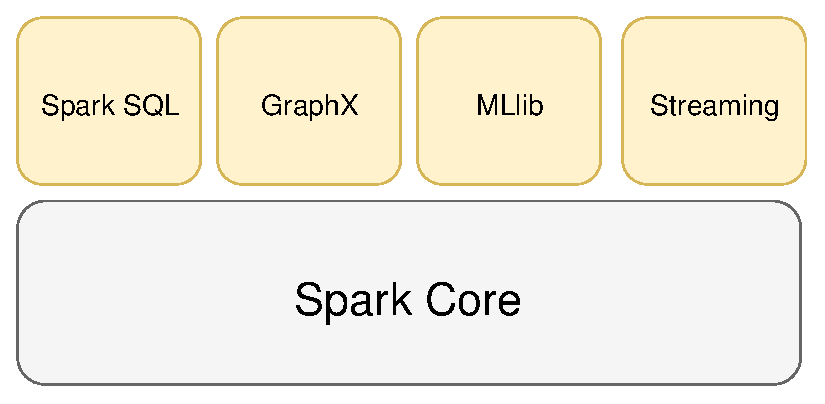
\includegraphics[width=0.7\textwidth]{img/sparkModules}
  \caption{Moduły Spark}
  \label{fig:SparkModules}
\end{figure}
\subsubsection*{Spark SQL}
Moduł dodający możliwość operowania na danych wykorzystywanych przez Sparka za pomocą języka SQL.
Pochodzenie danych nie ma znaczenia. Mogą być umieszone w
relacyjnych bazach danych, NoSQL, JSON, CSV czy innych ustrukturyzowanych formatach.
Szczegóły implementacyjne są skutecznie ukrywane.

Spark SQL można bezproblemowo wykorzystywać razem z innymi modułami (Spark Streaming, Spark ML czy GraphX).
Może być wykorzystywany zarówno w przetwarzaniu wsadowym historycznych danych
czy analizie strumieniowej w czasie rzeczywistym.
\subsubsection*{Spark GraphX}
Grapx dostarcza struktury danych umożliwiające na reprezentacje danych w formie grafów
zarówno sterowanych jak i niesterowanych.
Dodatkowo w tym module znajdują się przygotowana operatory i algorytmy umożliwiające prace z grafami.
\subsubsection*{Spark MLlib}
MLlib rozszerza Spark o dodatkowe funkcjonalności związane z uczeniem maszynowym (\textit{machine learning})
i analizą statystyczną.
Moduł ten zawiera wiele zaimplementowanych algorytmów między innymi do:
\begin{itemize}
  \item regresji liniowej (\textit{linear regression}),
  \item klasyfikatory Bayesa (\textit{Naive Bayes}),
  \item algorytmy do analizy skupień (\textit{cluster analysis}),
\end{itemize}
i wiele innych.
\subsubsection*{Spark Streaming}
Moduł Spark Streaming rozszerza podstawowe funkcjonalności o przetwarzanie strumieniowe danych.
Funkcjonalność przetwarzania strumieniowego zrealizowana jest poprzez mikro-buforowanie.
Strumień dzielony jest na mini-wsady o konfigurowalnym rozmiarze,
które dalej można przetwarzać za pomocą ogólnych (podstawowych) mechanizmów systemu Spark.

\subsection{Apache Storm}
Apache Storm jest framworkiem umożliwiającym strumieniowe przetwarzanie danych w czasie rzeczywistym.
Charakteryzuje się przy tym:
\begin{itemize}
  \item skalowalnością,
  \item odpornością na awarię,
  \item niezawodnością.
\end{itemize}
Stworzony został przez inżynierów z firmy
Backtype \footnote{\url{https://en.wikipedia.org/wiki/BackType}},
a po jej przejęciu, rozwijany przez inżynierów Twittera \footnote{\url{https://en.wikipedia.org/wiki/Twitter}}.
Obecnie projekt jest nadzworowany przez fundację Apache \footnote{\url{https://en.wikipedia.org/wiki/Apache_Software_Foundation}}.

Podobnie jak w przypadku Apache Storm zadanie jest odseparowane od wszelkich kwestii technicznych.

Centralnym punktem jest topologia (ang. \textit{topology}),
która reprezentuje zadanie w formie acyklicznego grafu skierowanego.
Graf ten ma 2 rodzaje węzłów.
\begin{itemize}
  \item \textit{Spouts} są źródłem danych w topologii.
  Pobierają je z zewnętrznego źródła i wprowadzają wewnątrz.
  \item \textit{Bolts} są miejscem,
  w którym następuje procesowanie danych: modyfikacja, filtracja czy agregacja.
\end{itemize}
Pomiędzy węzłami poruszają się krotki (ang. \textit{tuples}),
które są kontenerami na dane wyprodukawane przez węzły.
% budowa rysunek
\begin{figure}[htbp]
\centering
	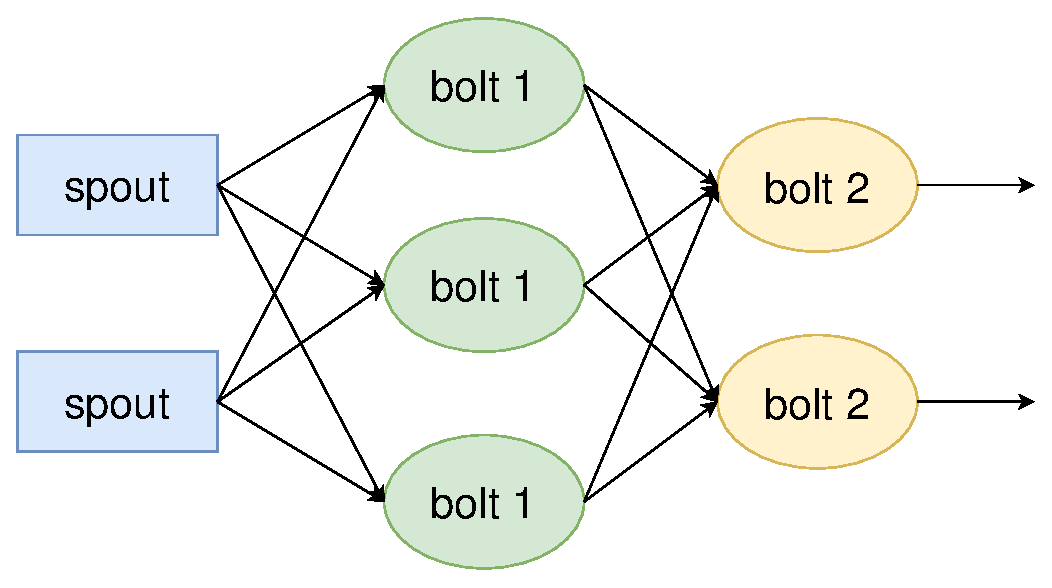
\includegraphics[width=1\textwidth]{img/storm}
	\caption{Topologia rozwiązania Apache Storm}
  \label{fig:StormTopology}
\end{figure}
% at least once
należy być przygotowanym,
że wiadomość może zostać przetworzona więcej niż jeden raz

